\documentclass[11pt,a4paper]{article}
\usepackage[margin=1in]{geometry}
\usepackage{amsmath,amssymb,amsthm}
\usepackage{mathtools}
\usepackage{enumitem}
\usepackage{xcolor}
\usepackage{tikz}
\usetikzlibrary{arrows.meta,decorations.markings}

% Custom commands for XYZ methodology
\newcommand{\stage}[1]{\textbf{\textcolor{blue}{#1}}}
\newcommand{\critical}[1]{\textbf{\textcolor{red}{#1}}}

\title{Exercise Sheet 1, Question 4: 1D Phase Portraits\\
Complete Solution with XYZ Methodology\\
Methods of Applied Mathematics [SEMT30006]}
\author{}
\date{}

\begin{document}

\maketitle

\section*{Problem Statement}

Sketch phase portraits for the following differential equations, and describe the long-time behaviour for the given starting conditions.

\begin{enumerate}[label=(\alph*)]
    \item $\frac{du}{dt} = \frac{2}{1+u^2} - 1$, with $u(0) = -2$, $u(0) = 0$ and $u(0) = 2$.
    \item $\frac{du}{dt} = u^3 + 5u^2 - 6u$, with $u(0) = -1$ and $u(0) = 4$.
\end{enumerate}

\section{Foundational Concepts: 1D Phase Portraits}

\subsection*{What is a Phase Portrait?}

\begin{itemize}[leftmargin=*]
\item \stage{STAGE X (Definition):}
A \textbf{phase portrait} is a geometric representation of the trajectories of a dynamical system in the phase space. For 1D systems $\frac{du}{dt} = f(u)$:
\begin{itemize}
    \item The \textbf{phase space} is the $u$-axis (one dimension)
    \item \textbf{Equilibria} (fixed points) occur where $f(u) = 0$
    \item The \textbf{flow} is represented by arrows showing direction of motion
    \item Trajectories are solution curves $u(t)$ plotted against $u$
\end{itemize}

\item \stage{STAGE Y (Why phase portraits are useful):}
Phase portraits provide qualitative understanding without solving explicitly:
\begin{enumerate}
    \item Identify all equilibria quickly
    \item Determine stability (stable/unstable)
    \item Predict long-time behavior from any initial condition
    \item Visualize the global dynamics
\end{enumerate}

\item \stage{STAGE Z (How to construct):}
\begin{enumerate}
    \item Find equilibria: solve $f(u) = 0$
    \item Determine flow direction: check sign of $f(u)$ in each region
    \begin{itemize}
        \item $f(u) > 0$: flow to the right ($u$ increases)
        \item $f(u) < 0$: flow to the left ($u$ decreases)
    \end{itemize}
    \item Classify equilibria:
    \begin{itemize}
        \item $f'(u^*) < 0$: stable (attractor)
        \item $f'(u^*) > 0$: unstable (repeller)
    \end{itemize}
    \item Draw arrows and trajectories
\end{enumerate}
\end{itemize}

\critical{KEY PRINCIPLE:} For 1D autonomous systems, solutions can never cross. Time flows monotonically along the phase line, and trajectories either approach equilibria or diverge to $\pm\infty$.

\newpage

\section{Part (a): $\frac{du}{dt} = \frac{2}{1+u^2} - 1$}

\subsection*{Step 1: Find Equilibria}

\begin{itemize}[leftmargin=*]
\item \stage{STAGE X (Setting up equilibrium equation):}
Equilibria occur where $\frac{du}{dt} = 0$:
\begin{align}
\frac{2}{1+u^2} - 1 = 0
\end{align}

\item \stage{STAGE Y (Solving for equilibria):}
\begin{align}
\frac{2}{1+u^2} &= 1 \\
2 &= 1 + u^2 \\
u^2 &= 1 \\
u &= \pm 1
\end{align}

\item \stage{STAGE Z (Equilibrium points):}
\begin{align}
\boxed{u^*_1 = -1, \quad u^*_2 = +1}
\end{align}

There are exactly two equilibria.
\end{itemize}

\subsection*{Step 2: Determine Flow Direction}

\begin{itemize}[leftmargin=*]
\item \stage{STAGE X (Define the function):}
Let $f(u) = \frac{2}{1+u^2} - 1$.

We need to determine the sign of $f(u)$ in each region:
\begin{itemize}
    \item Region I: $u < -1$
    \item Region II: $-1 < u < 1$
    \item Region III: $u > 1$
\end{itemize}

\item \stage{STAGE Y (Test points in each region):}

\textbf{Region I: $u < -1$} (test at $u = -2$):
\begin{align}
f(-2) = \frac{2}{1+4} - 1 = \frac{2}{5} - 1 = -\frac{3}{5} < 0
\end{align}
Flow to the LEFT ($\leftarrow$)

\textbf{Region II: $-1 < u < 1$} (test at $u = 0$):
\begin{align}
f(0) = \frac{2}{1+0} - 1 = 2 - 1 = 1 > 0
\end{align}
Flow to the RIGHT ($\rightarrow$)

\textbf{Region III: $u > 1$} (test at $u = 2$):
\begin{align}
f(2) = \frac{2}{1+4} - 1 = \frac{2}{5} - 1 = -\frac{3}{5} < 0
\end{align}
Flow to the LEFT ($\leftarrow$)

\item \stage{STAGE Z (Flow pattern):}
\begin{align}
u < -1: & \quad f(u) < 0 \quad (\text{decreasing}) \\
-1 < u < 1: & \quad f(u) > 0 \quad (\text{increasing}) \\
u > 1: & \quad f(u) < 0 \quad (\text{decreasing})
\end{align}
\end{itemize}

\subsection*{Step 3: Classify Equilibria Stability}

\begin{itemize}[leftmargin=*]
\item \stage{STAGE X (Method 1: Flow direction analysis):}

At $u^* = -1$:
\begin{itemize}
    \item Just left ($u < -1$): flow is $\leftarrow$ (away)
    \item Just right ($u > -1$): flow is $\rightarrow$ (away)
\end{itemize}
Both sides flow \textbf{away} from $u^* = -1$ $\Rightarrow$ \textbf{UNSTABLE}

At $u^* = +1$:
\begin{itemize}
    \item Just left ($u < 1$): flow is $\rightarrow$ (toward)
    \item Just right ($u > 1$): flow is $\leftarrow$ (toward)
\end{itemize}
Both sides flow \textbf{toward} $u^* = +1$ $\Rightarrow$ \textbf{STABLE}

\item \stage{STAGE Y (Method 2: Linear stability analysis):}
Compute $f'(u)$:
\begin{align}
f'(u) = \frac{d}{du}\left(\frac{2}{1+u^2} - 1\right) = -\frac{4u}{(1+u^2)^2}
\end{align}

At $u^* = -1$:
\begin{align}
f'(-1) = -\frac{4(-1)}{(1+1)^2} = \frac{4}{4} = 1 > 0 \quad \Rightarrow \quad \textbf{UNSTABLE}
\end{align}

At $u^* = +1$:
\begin{align}
f'(+1) = -\frac{4(1)}{(1+1)^2} = -\frac{4}{4} = -1 < 0 \quad \Rightarrow \quad \textbf{STABLE}
\end{align}

\item \stage{STAGE Z (Summary):}
\begin{align}
u^* = -1: & \quad \text{Unstable equilibrium (repeller)} \\
u^* = +1: & \quad \text{Stable equilibrium (attractor)}
\end{align}
\end{itemize}

\subsection*{Step 4: Sketch Phase Portrait}

\begin{itemize}[leftmargin=*]
\item \stage{STAGE X (Phase line diagram):}

\begin{center}
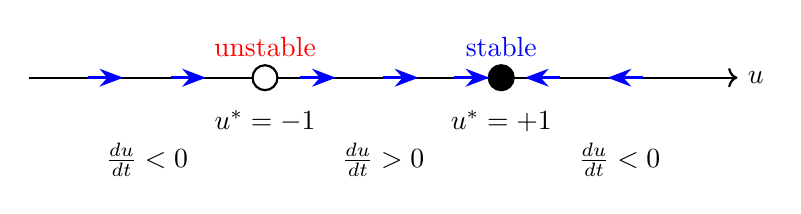
\begin{tikzpicture}[scale=1.5]
    % Draw the main axis
    \draw[->,thick] (-3,0) -- (3,0) node[right] {$u$};

    % Mark equilibria
    \draw[fill=white,thick] (-1,0) circle (3pt) node[below=8pt] {$u^*=-1$};
    \draw[fill=black,thick] (1,0) circle (3pt) node[below=8pt] {$u^*=+1$};

    % Add labels
    \node[above] at (-1,0.1) {\textcolor{red}{unstable}};
    \node[above] at (1,0.1) {\textcolor{blue}{stable}};

    % Draw flow arrows
    % Region I: u < -1
    \draw[-{Stealth[length=3mm]},very thick,blue] (-2.5,0) -- (-2.2,0);
    \draw[-{Stealth[length=3mm]},very thick,blue] (-1.8,0) -- (-1.5,0);

    % Region II: -1 < u < 1
    \draw[-{Stealth[length=3mm]},very thick,blue] (-0.7,0) -- (-0.4,0);
    \draw[-{Stealth[length=3mm]},very thick,blue] (0,0) -- (0.3,0);
    \draw[-{Stealth[length=3mm]},very thick,blue] (0.6,0) -- (0.9,0);

    % Region III: u > 1
    \draw[-{Stealth[length=3mm]},very thick,blue] (1.5,0) -- (1.2,0);
    \draw[-{Stealth[length=3mm]},very thick,blue] (2.2,0) -- (1.9,0);

    % Region labels
    \node[below=20pt] at (-2,0) {$\frac{du}{dt} < 0$};
    \node[below=20pt] at (0,0) {$\frac{du}{dt} > 0$};
    \node[below=20pt] at (2,0) {$\frac{du}{dt} < 0$};
\end{tikzpicture}
\end{center}

\item \stage{STAGE Y (Interpretation):}
\begin{itemize}
    \item Open circle at $u=-1$: unstable equilibrium (repeller)
    \item Filled circle at $u=+1$: stable equilibrium (attractor)
    \item Arrows show flow direction
    \item All trajectories eventually approach $u=+1$ (except starting exactly at $u=-1$)
\end{itemize}

\item \stage{STAGE Z (Global dynamics):}
The system has a single basin of attraction at $u^* = +1$, attracting all trajectories except the unstable equilibrium at $u^* = -1$.
\end{itemize}

\subsection*{Step 5: Analyze Specific Initial Conditions}

\begin{itemize}[leftmargin=*]
\item \stage{STAGE X (Three initial conditions):}

\textbf{Case 1: $u(0) = -2$}
\begin{itemize}
    \item Starting position: $u = -2$ (in region $u < -1$)
    \item Flow direction: $\leftarrow$ (decreasing)
    \item Long-time behavior: $u(t) \to -\infty$ as $t \to \infty$
\end{itemize}

\textbf{Case 2: $u(0) = 0$}
\begin{itemize}
    \item Starting position: $u = 0$ (in region $-1 < u < 1$)
    \item Flow direction: $\rightarrow$ (increasing)
    \item Long-time behavior: $u(t) \to +1$ as $t \to \infty$
\end{itemize}

\textbf{Case 3: $u(0) = 2$}
\begin{itemize}
    \item Starting position: $u = 2$ (in region $u > 1$)
    \item Flow direction: $\leftarrow$ (decreasing)
    \item Long-time behavior: $u(t) \to +1$ as $t \to \infty$
\end{itemize}

\item \stage{STAGE Y (Detailed trajectory behavior):}

\textbf{Trajectory from $u(0) = -2$:}
\begin{align}
u(t): \quad -2 \to -3 \to -4 \to \cdots \to -\infty
\end{align}
This trajectory escapes to $-\infty$. Since $f(u) \approx -1$ for large $|u|$, the escape rate is approximately linear: $u(t) \approx u_0 - t$.

\textbf{Trajectory from $u(0) = 0$:}
\begin{align}
u(t): \quad 0 \to 0.5 \to 0.8 \to 0.95 \to \cdots \to 1^-
\end{align}
This trajectory monotonically approaches $u^* = +1$ from below. Near equilibrium, $u(t) \approx 1 - Ce^{-t}$ (exponential approach).

\textbf{Trajectory from $u(0) = 2$:}
\begin{align}
u(t): \quad 2 \to 1.5 \to 1.2 \to 1.05 \to \cdots \to 1^+
\end{align}
This trajectory monotonically approaches $u^* = +1$ from above. Near equilibrium, $u(t) \approx 1 + Ce^{-t}$.

\item \stage{STAGE Z (Summary of long-time behavior):}
\begin{align}
u(0) = -2: & \quad u(t) \to -\infty \quad \text{(diverges)} \\
u(0) = 0: & \quad u(t) \to +1 \quad \text{(converges to stable equilibrium)} \\
u(0) = 2: & \quad u(t) \to +1 \quad \text{(converges to stable equilibrium)}
\end{align}
\end{itemize}

\subsection*{Step 6: Separatrix and Basin of Attraction}

\begin{itemize}[leftmargin=*]
\item \stage{STAGE X (Separatrix):}
The \textbf{separatrix} is the boundary between different long-time behaviors. In this system:
\begin{itemize}
    \item The unstable equilibrium $u^* = -1$ acts as a separatrix
    \item Initial conditions $u_0 > -1$ converge to $u^* = +1$
    \item Initial conditions $u_0 < -1$ diverge to $-\infty$
\end{itemize}

\item \stage{STAGE Y (Basin of attraction):}
The \textbf{basin of attraction} for $u^* = +1$ is:
\begin{align}
\mathcal{B}(u^* = +1) = (-1, +\infty)
\end{align}

All initial conditions in this interval converge to the stable equilibrium.

\item \stage{STAGE Z (Physical interpretation):}
This system exhibits a threshold behavior:
\begin{itemize}
    \item Above threshold ($u > -1$): system stabilizes at $u = +1$
    \item Below threshold ($u < -1$): system escapes to $-\infty$
    \item At threshold ($u = -1$): unstable balance
\end{itemize}
\end{itemize}

\critical{KEY INSIGHT:} The unstable equilibrium at $u^* = -1$ is the critical threshold separating bounded behavior (convergence to $u^*=+1$) from unbounded behavior (divergence to $-\infty$).

\subsection*{Step 7: Time Evolution (Qualitative)}

\begin{itemize}[leftmargin=*]
\item \stage{STAGE X (Sketch of $u(t)$ vs $t$):}

\begin{center}
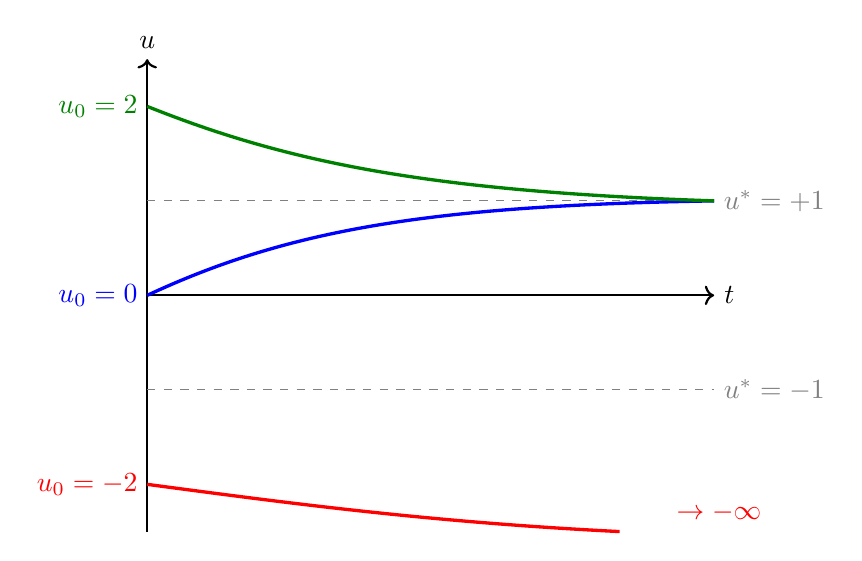
\begin{tikzpicture}[scale=1.2]
    % Axes
    \draw[->,thick] (0,0) -- (6,0) node[right] {$t$};
    \draw[->,thick] (0,-2.5) -- (0,2.5) node[above] {$u$};

    % Equilibria lines
    \draw[dashed,gray] (0,1) -- (6,1) node[right] {$u^*=+1$};
    \draw[dashed,gray] (0,-1) -- (6,-1) node[right] {$u^*=-1$};

    % Trajectory from u(0) = -2 (diverges)
    \draw[very thick,red] (0,-2) .. controls (1.5,-2.2) and (3,-2.4) .. (5,-2.5);
    \node[left,red] at (0,-2) {$u_0=-2$};

    % Trajectory from u(0) = 0 (converges from below)
    \draw[very thick,blue] (0,0) .. controls (1.5,0.7) and (3,0.95) .. (6,1);
    \node[left,blue] at (0,0) {$u_0=0$};

    % Trajectory from u(0) = 2 (converges from above)
    \draw[very thick,green!50!black] (0,2) .. controls (1.5,1.4) and (3,1.1) .. (6,1);
    \node[left,green!50!black] at (0,2) {$u_0=2$};

    % Labels
    \node[right] at (5.5,-2.3) {\textcolor{red}{$\to -\infty$}};
\end{tikzpicture}
\end{center}

\item \stage{STAGE Y (Rates of convergence/divergence):}

For $u_0 = 0$ or $u_0 = 2$ approaching $u^* = +1$:
\begin{itemize}
    \item Near equilibrium: $|u(t) - 1| \sim e^{-t}$ (exponential)
    \item Rate constant: $|f'(+1)| = 1$
    \item Time scale: $\tau = 1$ (reaches $\approx 63\%$ of final value in time $\tau$)
\end{itemize}

For $u_0 = -2$ diverging to $-\infty$:
\begin{itemize}
    \item Far from equilibria: $f(u) \approx -1$ (approximately constant)
    \item Divergence rate: $u(t) \approx u_0 - t$ (approximately linear)
\end{itemize}

\item \stage{STAGE Z (Summary):}
\begin{itemize}
    \item Two trajectories converge exponentially to stable equilibrium
    \item One trajectory diverges approximately linearly to $-\infty$
    \item The unstable equilibrium at $u^*=-1$ separates these behaviors
\end{itemize}
\end{itemize}

\newpage

\section{Part (b): $\frac{du}{dt} = u^3 + 5u^2 - 6u$}

\subsection*{Step 1: Find Equilibria}

\begin{itemize}[leftmargin=*]
\item \stage{STAGE X (Setting up equilibrium equation):}
Equilibria occur where $\frac{du}{dt} = 0$:
\begin{align}
u^3 + 5u^2 - 6u = 0
\end{align}

\item \stage{STAGE Y (Factoring):}
Factor out $u$:
\begin{align}
u(u^2 + 5u - 6) = 0
\end{align}

This gives $u = 0$ or $u^2 + 5u - 6 = 0$.

For the quadratic, use the quadratic formula or factor:
\begin{align}
u^2 + 5u - 6 = (u + 6)(u - 1) = 0
\end{align}

So $u = -6$ or $u = 1$.

\item \stage{STAGE Z (Three equilibria):}
\begin{align}
\boxed{u^*_1 = -6, \quad u^*_2 = 0, \quad u^*_3 = +1}
\end{align}

There are exactly three equilibria, ordered: $-6 < 0 < 1$.
\end{itemize}

\subsection*{Step 2: Rewrite in Factored Form}

\begin{itemize}[leftmargin=*]
\item \stage{STAGE X (Factored form):}
\begin{align}
\frac{du}{dt} = u(u+6)(u-1)
\end{align}

\item \stage{STAGE Y (Why factored form is useful):}
The sign of $f(u) = u(u+6)(u-1)$ depends on the signs of each factor:
\begin{itemize}
    \item $u$: negative for $u < 0$, positive for $u > 0$
    \item $(u+6)$: negative for $u < -6$, positive for $u > -6$
    \item $(u-1)$: negative for $u < 1$, positive for $u > 1$
\end{itemize}

\item \stage{STAGE Z (Sign analysis regions):}
We have 4 regions separated by the three equilibria:
\begin{itemize}
    \item Region I: $u < -6$
    \item Region II: $-6 < u < 0$
    \item Region III: $0 < u < 1$
    \item Region IV: $u > 1$
\end{itemize}
\end{itemize}

\subsection*{Step 3: Determine Flow Direction}

\begin{itemize}[leftmargin=*]
\item \stage{STAGE X (Sign table method):}

\begin{center}
\begin{tabular}{|c|c|c|c|c|}
\hline
\textbf{Region} & $u$ & $(u+6)$ & $(u-1)$ & $f(u) = u(u+6)(u-1)$ \\
\hline
$u < -6$ & $-$ & $-$ & $-$ & $(-)(-)(-)= -$ \\
\hline
$-6 < u < 0$ & $-$ & $+$ & $-$ & $(-)(+)(-) = +$ \\
\hline
$0 < u < 1$ & $+$ & $+$ & $-$ & $(+)(+)(-) = -$ \\
\hline
$u > 1$ & $+$ & $+$ & $+$ & $(+)(+)(+) = +$ \\
\hline
\end{tabular}
\end{center}

\item \stage{STAGE Y (Flow directions):}

\textbf{Region I: $u < -6$} (e.g., $u = -7$):
\begin{align}
f(-7) = (-7)(-1)(-8) = -56 < 0 \quad \Rightarrow \quad \text{flow LEFT } (\leftarrow)
\end{align}

\textbf{Region II: $-6 < u < 0$} (e.g., $u = -3$):
\begin{align}
f(-3) = (-3)(3)(-4) = 36 > 0 \quad \Rightarrow \quad \text{flow RIGHT } (\rightarrow)
\end{align}

\textbf{Region III: $0 < u < 1$} (e.g., $u = 0.5$):
\begin{align}
f(0.5) = (0.5)(6.5)(-0.5) = -1.625 < 0 \quad \Rightarrow \quad \text{flow LEFT } (\leftarrow)
\end{align}

\textbf{Region IV: $u > 1$} (e.g., $u = 2$):
\begin{align}
f(2) = (2)(8)(1) = 16 > 0 \quad \Rightarrow \quad \text{flow RIGHT } (\rightarrow)
\end{align}

\item \stage{STAGE Z (Summary of flow):}
\begin{align}
u < -6: & \quad f(u) < 0 \quad (\text{decreasing}) \\
-6 < u < 0: & \quad f(u) > 0 \quad (\text{increasing}) \\
0 < u < 1: & \quad f(u) < 0 \quad (\text{decreasing}) \\
u > 1: & \quad f(u) > 0 \quad (\text{increasing})
\end{align}
\end{itemize}

\subsection*{Step 4: Classify Equilibria Stability}

\begin{itemize}[leftmargin=*]
\item \stage{STAGE X (Flow analysis at each equilibrium):}

At $u^* = -6$:
\begin{itemize}
    \item Just left ($u < -6$): flow is $\leftarrow$ (away)
    \item Just right ($u > -6$): flow is $\rightarrow$ (away)
\end{itemize}
Both sides flow away $\Rightarrow$ \textbf{UNSTABLE}

At $u^* = 0$:
\begin{itemize}
    \item Just left ($u < 0$): flow is $\rightarrow$ (toward)
    \item Just right ($u > 0$): flow is $\leftarrow$ (toward)
\end{itemize}
Both sides flow toward $\Rightarrow$ \textbf{STABLE}

At $u^* = +1$:
\begin{itemize}
    \item Just left ($u < 1$): flow is $\leftarrow$ (away)
    \item Just right ($u > 1$): flow is $\rightarrow$ (away)
\end{itemize}
Both sides flow away $\Rightarrow$ \textbf{UNSTABLE}

\item \stage{STAGE Y (Linear stability verification):}
Compute $f'(u)$:
\begin{align}
f(u) &= u^3 + 5u^2 - 6u \\
f'(u) &= 3u^2 + 10u - 6
\end{align}

At $u^* = -6$:
\begin{align}
f'(-6) = 3(36) + 10(-6) - 6 = 108 - 60 - 6 = 42 > 0 \quad \Rightarrow \quad \textbf{UNSTABLE}
\end{align}

At $u^* = 0$:
\begin{align}
f'(0) = 3(0) + 10(0) - 6 = -6 < 0 \quad \Rightarrow \quad \textbf{STABLE}
\end{align}

At $u^* = +1$:
\begin{align}
f'(+1) = 3(1) + 10(1) - 6 = 3 + 10 - 6 = 7 > 0 \quad \Rightarrow \quad \textbf{UNSTABLE}
\end{align}

\item \stage{STAGE Z (Classification summary):}
\begin{align}
u^* = -6: & \quad \text{Unstable equilibrium (repeller)} \\
u^* = 0: & \quad \text{Stable equilibrium (attractor)} \\
u^* = +1: & \quad \text{Unstable equilibrium (repeller)}
\end{align}

The pattern is: unstable-stable-unstable.
\end{itemize}

\subsection*{Step 5: Sketch Phase Portrait}

\begin{itemize}[leftmargin=*]
\item \stage{STAGE X (Phase line diagram):}

\begin{center}
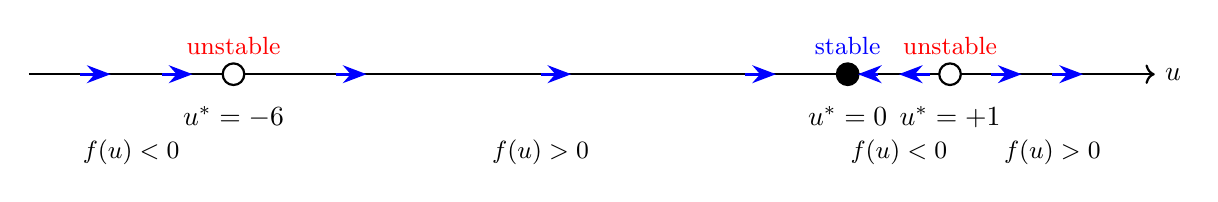
\begin{tikzpicture}[scale=1.3]
    % Draw the main axis
    \draw[->,thick] (-8,0) -- (3,0) node[right] {$u$};

    % Mark equilibria
    \draw[fill=white,thick] (-6,0) circle (3pt) node[below=8pt] {$u^*=-6$};
    \draw[fill=black,thick] (0,0) circle (3pt) node[below=8pt] {$u^*=0$};
    \draw[fill=white,thick] (1,0) circle (3pt) node[below=8pt] {$u^*=+1$};

    % Add labels
    \node[above] at (-6,0.1) {\textcolor{red}{\small unstable}};
    \node[above] at (0,0.1) {\textcolor{blue}{\small stable}};
    \node[above] at (1,0.1) {\textcolor{red}{\small unstable}};

    % Draw flow arrows
    % Region I: u < -6
    \draw[-{Stealth[length=3mm]},very thick,blue] (-7.5,0) -- (-7.2,0);
    \draw[-{Stealth[length=3mm]},very thick,blue] (-6.7,0) -- (-6.4,0);

    % Region II: -6 < u < 0
    \draw[-{Stealth[length=3mm]},very thick,blue] (-5,0) -- (-4.7,0);
    \draw[-{Stealth[length=3mm]},very thick,blue] (-3,0) -- (-2.7,0);
    \draw[-{Stealth[length=3mm]},very thick,blue] (-1,0) -- (-0.7,0);

    % Region III: 0 < u < 1
    \draw[-{Stealth[length=3mm]},very thick,blue] (0.8,0) -- (0.5,0);
    \draw[-{Stealth[length=3mm]},very thick,blue] (0.3,0) -- (0.1,0);

    % Region IV: u > 1
    \draw[-{Stealth[length=3mm]},very thick,blue] (1.4,0) -- (1.7,0);
    \draw[-{Stealth[length=3mm]},very thick,blue] (2,0) -- (2.3,0);

    % Region labels
    \node[below=20pt] at (-7,0) {\small $f(u) < 0$};
    \node[below=20pt] at (-3,0) {\small $f(u) > 0$};
    \node[below=20pt] at (0.5,0) {\small $f(u) < 0$};
    \node[below=20pt] at (2,0) {\small $f(u) > 0$};
\end{tikzpicture}
\end{center}

\item \stage{STAGE Y (Interpretation):}
\begin{itemize}
    \item Open circles at $u=-6$ and $u=+1$: unstable equilibria
    \item Filled circle at $u=0$: stable equilibrium (attractor)
    \item Arrows show flow direction in each region
\end{itemize}

\item \stage{STAGE Z (Global structure):}
The system has:
\begin{itemize}
    \item One stable equilibrium at $u^* = 0$ with basin of attraction $(-6, +1)$
    \item Two unstable equilibria acting as separatrices
    \item Trajectories outside $[-6, +1]$ diverge to $\pm\infty$
\end{itemize}
\end{itemize}

\subsection*{Step 6: Analyze Specific Initial Conditions}

\begin{itemize}[leftmargin=*]
\item \stage{STAGE X (Two initial conditions):}

\textbf{Case 1: $u(0) = -1$}
\begin{itemize}
    \item Starting position: $u = -1$ (in region $-6 < u < 0$)
    \item Flow direction: $\rightarrow$ (increasing)
    \item Path: $-1 \to -0.5 \to -0.1 \to \cdots \to 0^-$
    \item Long-time behavior: $u(t) \to 0$ as $t \to \infty$
\end{itemize}

\textbf{Case 2: $u(0) = 4$}
\begin{itemize}
    \item Starting position: $u = 4$ (in region $u > 1$)
    \item Flow direction: $\rightarrow$ (increasing)
    \item Path: $4 \to 5 \to 10 \to 100 \to \cdots \to +\infty$
    \item Long-time behavior: $u(t) \to +\infty$ as $t \to \infty$
\end{itemize}

\item \stage{STAGE Y (Detailed trajectory analysis):}

\textbf{From $u(0) = -1$:}
\begin{itemize}
    \item Trajectory stays in region $(-6, 0)$
    \item Monotonically increases toward stable equilibrium $u^* = 0$
    \item Near equilibrium: $u(t) \approx -Ce^{-6t}$ (exponential approach)
    \item Decay rate: $|f'(0)| = 6$ (fast convergence)
    \item Time scale: $\tau = 1/6 \approx 0.167$
\end{itemize}

\textbf{From $u(0) = 4$:}
\begin{itemize}
    \item Trajectory starts beyond unstable equilibrium $u^* = 1$
    \item Flows away from $u^* = 1$ to the right
    \item Growth accelerates: $f(u) = u(u+6)(u-1)$ grows cubically for large $u$
    \item For large $u$: $f(u) \approx u^3$
    \item Divergence is finite-time: $\frac{du}{dt} \sim u^3$ leads to blow-up
\end{itemize}

\item \stage{STAGE Z (Finite-time blow-up for $u_0 = 4$):}

For $u > 1$, approximate $f(u) \approx u^3$ for large $u$:
\begin{align}
\frac{du}{dt} \approx u^3 \quad \Rightarrow \quad \frac{du}{u^3} \approx dt
\end{align}

Integrating:
\begin{align}
-\frac{1}{2u^2} \approx t + C
\end{align}

At $t = 0$: $C = -\frac{1}{2u_0^2}$

\begin{align}
-\frac{1}{2u^2} &= t - \frac{1}{2u_0^2} \\
\frac{1}{u^2} &= \frac{1}{u_0^2} - 2t \\
u(t) &= \frac{1}{\sqrt{\frac{1}{u_0^2} - 2t}}
\end{align}

This blows up at time $t^* = \frac{1}{2u_0^2}$.

For $u_0 = 4$:
\begin{align}
t^* = \frac{1}{2(16)} = \frac{1}{32} \approx 0.03125
\end{align}

The solution reaches $+\infty$ in finite time $t^* \approx 0.031$!
\end{itemize}

\subsection*{Step 7: Basin of Attraction and Separatrices}

\begin{itemize}[leftmargin=*]
\item \stage{STAGE X (Basin of attraction for $u^* = 0$):}
\begin{align}
\mathcal{B}(u^* = 0) = (-6, +1)
\end{align}

All initial conditions in this open interval converge to $u^* = 0$.

\item \stage{STAGE Y (Separatrices):}
The unstable equilibria act as separatrices:
\begin{itemize}
    \item $u^* = -6$ separates:
    \begin{itemize}
        \item $u_0 < -6$: divergence to $-\infty$
        \item $u_0 > -6$: bounded behavior
    \end{itemize}
    \item $u^* = +1$ separates:
    \begin{itemize}
        \item $u_0 < 1$: convergence to $u^* = 0$ (if $u_0 > -6$)
        \item $u_0 > 1$: divergence to $+\infty$
    \end{itemize}
\end{itemize}

\item \stage{STAGE Z (Complete classification by initial condition):}
\begin{align}
u_0 < -6: & \quad u(t) \to -\infty \\
u_0 = -6: & \quad u(t) = -6 \text{ (stays at unstable equilibrium)} \\
-6 < u_0 < 1: & \quad u(t) \to 0 \\
u_0 = 1: & \quad u(t) = 1 \text{ (stays at unstable equilibrium)} \\
u_0 > 1: & \quad u(t) \to +\infty \text{ (finite-time blow-up)}
\end{align}
\end{itemize}

\subsection*{Step 8: Time Evolution Sketch}

\begin{itemize}[leftmargin=*]
\item \stage{STAGE X (Plot of $u(t)$ vs $t$):}

\begin{center}
\begin{tikzpicture}[scale=1.2]
    % Axes
    \draw[->,thick] (0,-7) -- (0,5) node[above] {$u$};
    \draw[->,thick] (0,0) -- (6,0) node[right] {$t$};

    % Equilibria lines
    \draw[dashed,gray] (0,0) -- (6,0) node[right] {$u^*=0$};
    \draw[dashed,gray] (0,-6) -- (6,-6) node[right] {$u^*=-6$};
    \draw[dashed,gray] (0,1) -- (6,1) node[right] {$u^*=+1$};

    % Trajectory from u(0) = -1 (converges to 0)
    \draw[very thick,blue] (0,-1) .. controls (1.5,-0.3) and (3,-0.05) .. (6,0);
    \node[left,blue] at (0,-1) {$u_0=-1$};

    % Trajectory from u(0) = 4 (blows up)
    \draw[very thick,red] (0,4) .. controls (0.15,4.5) and (0.25,5) .. (0.5,5);
    \draw[red,dashed,thick] (0.5,5) -- (0.5,4.8);
    \node[left,red] at (0,4) {$u_0=4$};
    \node[red,right] at (0.5,4.5) {blow-up at $t \approx 0.03$};

    % Vertical line at blow-up time
    \draw[red,dotted] (0.5,-7) -- (0.5,5);
\end{tikzpicture}
\end{center}

\item \stage{STAGE Y (Key features):}
\begin{itemize}
    \item Blue curve ($u_0 = -1$): smooth exponential convergence to $u^* = 0$
    \item Red curve ($u_0 = 4$): rapid divergence to $+\infty$ in finite time
    \item Vertical asymptote at blow-up time for $u_0 = 4$
\end{itemize}

\item \stage{STAGE Z (Summary):}
\begin{align}
u(0) = -1: & \quad u(t) \to 0 \text{ exponentially, } \tau = 1/6 \\
u(0) = 4: & \quad u(t) \to +\infty \text{ at } t \approx 0.031
\end{align}
\end{itemize}

\critical{KEY INSIGHT:} This system exhibits rich dynamics with a stable attractor at $u^*=0$ flanked by two unstable equilibria. Initial conditions outside the basin $(-6, +1)$ lead to finite-time blow-up, a phenomenon common in cubic nonlinearities.

\newpage

\section{Summary and Comparison}

\subsection*{Comparison of Parts (a) and (b)}

\begin{center}
\begin{tabular}{|l|c|c|}
\hline
\textbf{Feature} & \textbf{Part (a)} & \textbf{Part (b)} \\
\hline
Number of equilibria & 2 & 3 \\
\hline
Stable equilibria & 1 (at $u=+1$) & 1 (at $u=0$) \\
\hline
Unstable equilibria & 1 (at $u=-1$) & 2 (at $u=-6, +1$) \\
\hline
Basin of attraction & $(-1, +\infty)$ & $(-6, +1)$ \\
\hline
Divergence to $-\infty$ & Yes (if $u_0 < -1$) & Yes (if $u_0 < -6$) \\
\hline
Divergence to $+\infty$ & No & Yes (if $u_0 > +1$) \\
\hline
Finite-time blow-up & No & Yes (for $u_0 > 1$) \\
\hline
Nonlinearity & Rational function & Cubic polynomial \\
\hline
\end{tabular}
\end{center}

\subsection*{Key Lessons from 1D Phase Portraits}

\begin{itemize}[leftmargin=*]
\item \stage{STAGE X (What we learned):}
\begin{enumerate}
    \item \textbf{Equilibria classification:} Use flow direction or $f'(u^*)$ to determine stability
    \item \textbf{Separatrices:} Unstable equilibria separate regions with different long-time behavior
    \item \textbf{Basins of attraction:} The set of initial conditions leading to each attractor
    \item \textbf{Global structure:} Complete understanding of all possible trajectories
\end{enumerate}

\item \stage{STAGE Y (Techniques mastered):}
\begin{enumerate}
    \item Finding equilibria by solving $f(u) = 0$
    \item Determining flow direction using sign analysis
    \item Classifying stability using flow or derivatives
    \item Sketching phase portraits on the phase line
    \item Predicting long-time behavior from phase portraits
    \item Identifying finite-time blow-up
\end{enumerate}

\item \stage{STAGE Z (Connection to higher dimensions):}
In 1D:
\begin{itemize}
    \item Phase space is a line
    \item Trajectories can't cross
    \item Only nodes (stable/unstable) exist
    \item Analysis is completely solvable
\end{itemize}

In 2D (next question):
\begin{itemize}
    \item Phase space is a plane
    \item More complex equilibria: nodes, saddles, foci, centers
    \item Closed orbits (limit cycles) possible
    \item Richer dynamics, but still analyzable
\end{itemize}
\end{itemize}

\critical{UNIVERSAL PRINCIPLE:} In 1D autonomous systems, trajectories are monotonic between equilibria. Solutions either approach equilibria or diverge to $\pm\infty$. No oscillations or closed orbits are possible in 1D.

\vfill

\begin{center}
\Large\textbf{END OF QUESTION 4}
\end{center}

\end{document}
